\chapter{\iflanguage{ngerman}{Herausforderungen}{Challenges}}
\label{sec:overview}

Der Hybride OP-Saal bringt viele Vorteile für zukünftige Entwicklung des Operationssaals. Dennoch kommen bei der Planung, Umsetzung und Vernetzung einige Herausforderungen auf, die berücksichtigt werden müssen. 
Auch sind nicht alle Aspekte nur positiv und ob sich ein Hybrider OP-Saal tatsächlich lohnt, muss validiert werden.

\subsection{Nachteile}

Der Hybride OP-Saal weist sehr viele positive Aspekte auf, doch sind die negativen nicht zu vernachlässigen und werden deshalb im Folgenden besprochen.

Der Hybride OP-Saal wird in erster Linie durch die bildgebenden Verfahren definiert, doch wie bereits aus der Radiologie bekannt ist, müssen immer auch mögliche \glqq Mess-, Rekonstruktions- und Modellierungsfehler berücksichtigt werden\grqq{} \cite{DerDigitaleOperationssaal}. 
So können Partialvolumenartefakte (Abb \ref{fig:partial}) Grund dafür sein, dass Tumore in der falschen Größe dargestellt werden oder bei CT Bildern die besonders kleinen Läsionen (< 1cm) nicht in der Bildausgabe erkenntlich sind. Diese möglichen Fehler müssen in der Operationsplanung und späteren Ausführung berücksichtigt werden \cite{DerDigitaleOperationssaal}.

Hinzu kommt, dass Operationen im Hybriden OP-Saal teilweise unter laufender Röntgenkontrolle statt finden. Diese Strahlenbelastung betrifft nicht nur den Patienten sondern das gesamte behandelnde Team wird der durch den Patienten verursachten Streustrahlung ausgesetzt. Je nach Abstand, Winkel und Höhe zum Patienten während der Bildkontrolle, wird eine anwesende Person 9 bis 39\% der Strahlung ausgesetzt, die der Patient ausgesetzt wird (bei einem Patienten mit 65kg Körpergewicht). Je nach Größe und Gewicht des Patienten kann es aber auch zu einem höheren Streustrahlenanteil kommen und damit zu einer höheren Belastung für das behandelnde Team.
Nimmt man an, dass pro Operation durchschnittlich zwei 3D Scans gemacht werden, dann summiert sich die Strahlendosis für ein Teammitglied, bei 100 Operationen im Jahr, auf ungefähr 400µSv. Dies entspricht bereits 7\% der jährlichen maximalen Dosis und muss deshalb so weit wie möglich verhindert werden. Wenn immer möglich, sollte das Personal deshalb bei Bildaufnahmen hinter einer Strahlenschutzwand stehen oder den OP-Saal verlassen\cite{RadiationExposure}.

Ein anderes Problem entsteht beispielsweise bei der Tumorentfernung im Gehirn mit intraoperativem MRT. Um kleine Veränderungen (wie Brain Shift) frühzeitig erkennen und darauf reagieren zu können, sind viele regelmäßige Bildaufnahmen nötigt. Gleichzeitig muss für jede Bildaufnahme die Operation unterbrochen und für jedes Bild ein gewisser Zeitaufwand aufgebracht werden. Für ein iMR-Bild muss etwa mit einer Aufnahmezeit von circa 15 Minuten gerechnet werden \cite{BrainShiftInTumorResection}. Jede Aufnahme führt damit auch zu einer Verlängerung der Operationszeit und es muss somit ein Kompromiss zwischen Zeitaufwand und Bildhäufigkeit gefunden werden.\\
Alternativ besteht in diesem Fall immer auch noch die Möglichkeit, eine schlechtere Bildqualität in Kauf zu nehmen und dafür eine Aufnahmezeit von 5 Minuten, wenn man stattdessen zum US-Gerät greift. Dabei muss aber wiederum beachtet werden, dass Ultraschall, im Gegensatz zu Magnetresonanztomografie, nicht kontaktlos verwendet werden kann, was somit immer auch ein höheres Infektionsrisiko mit sich bringt \cite{BrainShiftInTumorResection}.

\begin{figure} [H]
	
\includegraphics[scale = 0.7]{Content/Pictures/partial.png}
	\caption{Beispiel für Partialvolumenartefakte: Links zeigt einen Tumor, die Mitte das finale Bild und rechts alle Voxel in denen Grauwerte des Tumors verzeichnet wurden \cite{DerDigitaleOperationssaal}}
	\label{fig:partial}
\end{figure}

\subsection{Kosten- Nutzen Verhältnis}

Eine der wichtigen Fragen die noch geklärt werden muss, ist ob ein Hybrider OP-Saal tatsächlich den Mehraufwand an Kosten und Umstrukturierung lohnt. Die benötigte Raumgröße und Ausrüstung führen dazu, dass ein Hybrider OP-Saal in der Anschaffung mehr als doppelt so teuer und in der Wartung fast doppelt so teuer wie ein konventioneller OP-Saal ist \cite{HybridOR}. \\
Gleichzeitig hat sich herausgestellt, dass neue medizinische Technologien meist positiv aufgenommen werden, obwohl ein Mehrwert dieser noch gar nicht bewiesen wurde. Dies und die Digitalisierung des Operationssaals, hat in den letzten Jahren zu erheblichen Steigerung der Gesundheitskosten beigetragen \cite{DerDigitaleOperationssaal}.

%TODO umformulieren, Fragen hab ich ja jetzt entfert
Weil die oben genannten Fragestellungen nicht wirklich beantwortet werden können, soll herausgearbeitet werden, welchen Mehrwert der Hybride OP-Saal tatsächlich bringt. Weil die Vorteile des Hybriden OP-Saals bereits im ersten Kapitel herausgearbeitet wurden, wird hier deshalb nur auf die Kosten und Operationszeit eingegangen.
% auf die Sterblichkeitsrate, Operationszeit und Kosten eingegangen.

Im Anwendungsfall des Bauchaortenaneurysma konnte eine Operationszeiteinsparung von 23,5 Minuten (von 120 auf 96,5 Minuten), mit einem Hybriden OP-Saal gegenüber einem konventionellen mit C-Bogen, erreicht werden. Die Zeiteinsparung führt zusätzlich auch zu einer Kosteneinsparung der Prozesskosten und beträgt 276,17€ weniger pro durchgeführte Operation.
Dieses Ergebnis muss jedoch kritisch betrachtet werden, da die Studie auf Ergebnissen eines konventionellen OPs mit 97 Patienten von 2007 bis 2010 und beim Hybriden mit 50 Patienten von 2012 bis 2015 durchgeführt wurde. Ein positiver Trend ist dennoch sehr wohl zu verzeichnen, da bei den Patienten und dem Operationsteam sehr auf  ähnliche Charakteristika geachtet wurde \cite{HybriderVsKonventioneller}.
Trotzdem können zwei so komplexe Systeme wie hier betrachtet, kaum miteinander verglichen werden. Trotz enormer Ähnlichkeiten wird immer einen gewisser Unterschied zwischen den verglichenen Patienten und Teams bleiben \cite{DerDigitaleOperationssaal}.

Dennoch ist durch die Operationszeiteinsparung im Hybriden OP-Saal eine Refinanzierung möglich \cite{HybriderVsKonventioneller}. Hinzu kommen positive Ergebnisse ohne einen direkten Vergleichswert, wie beispielsweise bei der Tumorentfernung. Bei 14 aus 16 Fällen konnten die Tumore komplett entfernt werden und mögliche auftretende Brain Shifts frühzeitig erkannt werden \cite{BrainShiftInTumorResection}.

Da Studien zum Vergleich zwischen einem Hybriden und Konventionellen Operationssaal zum einen kaum vorliegen und zum anderen schwierig durchzuführen und zu validieren sind, lässt sich die Frage zum tatsächlichen Nutzen sehr schwer beantworten. Hinzu kommt, dass man nicht einfach nur die Todesraten bei bestimmten Krankheitsbildern miteinander vergleichen kann, da diese teilweise sehr gering sind und sehr viele Probanden verglichen werden müssten, was in den meisten Fällen gar nicht möglich ist. Darüber hinaus geht eine verbesserte Überlebensrate nicht immer auch mit einer verbesserten Lebensqualität mit ein \cite{HybriderVsKonventioneller}. \\
Weitere wichtige Faktoren, die einen Einfluss auf den Nutzen haben, sind die gefühlte und tatsächliche Sicherheit von Patienten und Chirurgen. Die psychologische Seite ist jedoch noch viel schwieriger zu bewerten als das tatsächliche objektive Ergebnis \cite{DerDigitaleOperationssaal}.

Trotzdem lässt sich festhalten, dass der Hybride OP-Saal seine Vorteile mit sich bringt. Nicht in allen medizinischen Bereichen wird er einen gleichgroßen Nutzen zur Geltung bringen aber in denjenigen in denen er dies tut, eröffnen sich völlig neue Möglichkeiten zur Operationsdurchführung und somit stellt er die Zukunft des Operationssaals dar \cite{ORofTheFuture}.
%TODO Herausforderungen: auf  Brain Shift, Aortenaneurysma, Tumorentfernung und Herzchirurgie Todesrate wieder drauf eingehen wenn möglich

\subsection{Planung der Räumlichkeiten}

Die Raumplanung eines Hybriden OP-Saals ist ein sehr komplexer Prozess, da er mehreren Fachbereichen gerecht werden muss, die unterschiedliche und teilweise auch sich gegenseitig ausschließende Ansprüche haben. Aus diesem Grund müssen alle fachbereichsübergreifenden Chirurgen aber auch Anästhesisten, Arzthelfer und Techniker in den Planungsprozess miteinbezogen werden.
Gleichzeitig ist durch die erhöhte Anzahl an Mitgliedern (8 bis 20 Personen) im Operationsteam eine Raumgröße von circa 70m² empfehlenswert. Mit Kontroll-, Technik und Vorbereitungsraum müssen dann insgesamt mit circa 150m² gerechnet werden. Je nachdem ob die Geräte und Systeme wie der C-Bogen über eine Decken- oder Bodenbefestigung angebracht werden, müssen diese einem Gewicht von 650 bis 1800kg standhalten. Gleichzeitig dürfen die bildgebenden Systeme, Monitore, Beleuchtungsanlagen und das Personal nicht miteinander Kollidieren (Abb. \ref{fig:roomplanning}). Durch die große Raumgröße und Montage von Geräten an der Decke, wird zusätzlich noch die Einhaltung der Hygienevorschriften erschwert \cite{TechnicalConsiderations}.\\ 
Aus den genannten Gründen muss normalerweise mit einer relativ langen Planungsphase für einen Hybriden OP-Saal gerechnet werden, um allen Ansprüchen einigermaßen gerecht zu werden und einen zukunftsfähigen OP-Saal zu errichten.

\begin{figure} [H]
	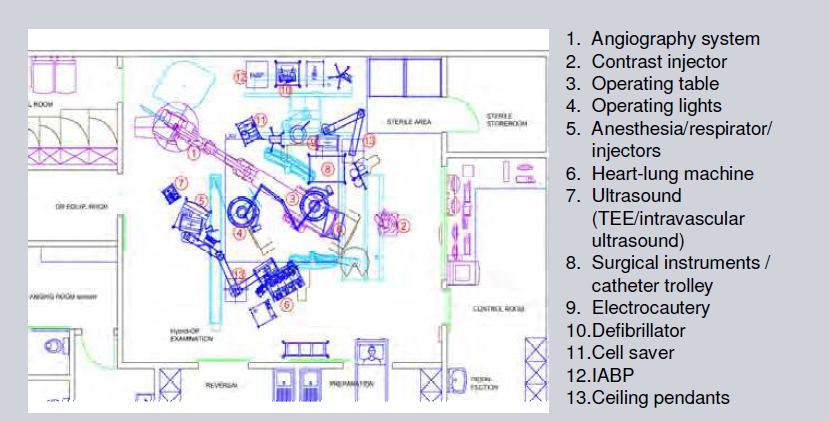
\includegraphics[scale = 0.7]{Content/Pictures/roomplanning.png}
	\caption{Beispielhaftes Layout für die Planung eines Hybriden OP-Saals \cite{HybridOR}}
	\label{fig:roomplanning}
\end{figure}


 





